\documentclass{article}

\usepackage[utf8]{inputenc}
\usepackage[margin=1in]{geometry}
\usepackage[titletoc,title]{appendix}
\usepackage{amsmath,amsfonts,amssymb,mathtools}
\usepackage{graphicx,float}
\usepackage[ruled,vlined]{algorithm2e}
\usepackage{algorithmic}\usepackage{minted}
\usemintedstyle{borland}

\usepackage{amsmath}

\usepackage{biblatex}
\addbibresource{references.bib}

% Title content
\title{\Large KEN 4154 Assignment 1 \\ \normalsize Backpropagation}
\author{Adrian Sondermann, Abel de Wit}
\date{November 3, 2020}

\begin{document}

\maketitle

% Introduction and Overview
\section{Introduction}
In this assignment we are tasked to write a neural network from scratch using no external libraries. The task at hand is training the network such that it is able to represent the input that is passed in the output layer as well, while going trough a middle/hidden layer that has less nodes than the in- and output layers.\newline

After this is implemented, we are asked to interpret the results of our network, including the convergence, the weights and
activations of the network, to see whether we can understand how the network learned to still represent these 8 input neurons trough the 3 hidden neurons. 

\section{Implementation}
The implementation strictly follows the algorithm described in the lectures slides and the help-file for backpropagation. A small change was made regarding the gradient descent: the weights get updated every time the $\Delta_{ij}^{l}$ are calculated, using a single training example. Therefore, the algorithm converged faster while testing, because the weights start to spread in different directions independently. Finally a learning curve containing the sum of squared output errors per iteration is returned.

The whole implementation is vectorised and in order to generate reproducible weights, the random generator of \texttt{numpy} is seeded with 0 initially. 

\section{Results}

\subsection{Tuning the parameters}
Using the implementation of the network, we created a simple GridSearch over the three tunable parameters \texttt{learningRate} (between 0.1 and 0.9),  \texttt{weightDecay} (between 0 and 0.5), and \texttt{iterations} (between 100 and 5000). 
One neural network was trained per unique parameter combination and the results were saved. All these combinations converge to a local minimum of the costs in the long run (possibly more than 5000 iterations needed!). Due to the independence of a single weight update on 7 training examples, the cumulative errors may fluctuate before finally converging to a local minimum.

From this GridSearch the best parameters were derived, which are given in Table \ref{tab:opt_params} and result in a error of approximately 0.000019. The learning rates (errors) are visualized in Figure \ref{fig:gs_errors}.

Another aspect to pay attention to is the choice of the \texttt{weightDecay} parameter, as nonzero values result in an training error rate always above 0. Because the training data is noise-free, using no \texttt{weightDecay} yields the lowest error.

\begin{table}
    \centering
    \begin{tabular}{l|c}
        parameter & value \\
        \hline
        learningRate & 0.9 \\
        weightDecay & 0 \\
        iterations & 5000 \\
    \end{tabular}
    \caption{Optimal parameters by GridSearch}
    \label{tab:opt_params}
\end{table}

\begin{figure}
    \centering
    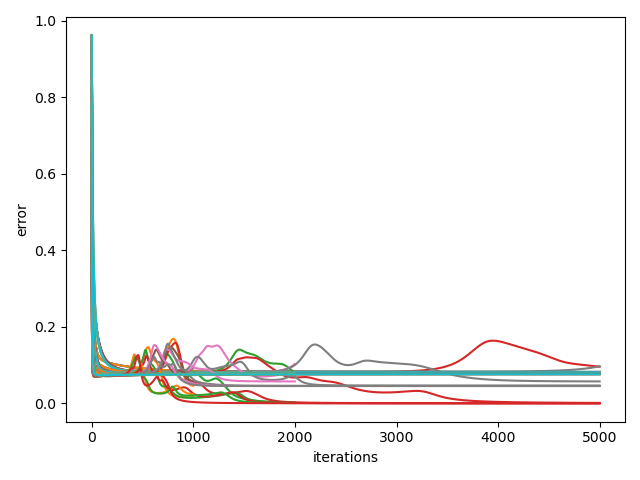
\includegraphics[width=0.6\textwidth]{gs_errors.png}
    \caption{Learning curves of all models}
    \label{fig:gs_errors}
\end{figure}

\subsection{Analysis}

Using specific parameters, the program can be executed to analyse the network with respect to the weights. For the values from Table \ref{tab:opt_params} the final weights in the hidden and output layer are presented in Figures \ref{fig:weights_hidden} and \ref{fig:weights_output}. The x-axis contains the bias (0) and the weights which will be used to calculate the activations of the neurons presented by the y-axis. Positive and negative weights are colored distinctively. According to those colors, every input is binary ''encoded'' by the hidden layer and ''decoded'' by the output layer. This results in weight matrices (without biases), which are transposed versions of another, if the values are seen as binary (smaller/bigger than 0). Because of this, the visualized network looks symmetrical along the hidden layer, as visualized in Figure \ref{fig:NN_visualized}.

Moreover, as the input and output can be viewed as binary data the following can be assumed: as

\begin{equation}
    \#possibleValues^{\#hiddenNotes} = 2^3 = 8 = \#inputs = \#outputs    
\end{equation}

holds, the whole assignment could not be solved with 2 hidden nodes, if a low error rate is desired. If less output nodes are used the number of internal nodes could be reduced.

\begin{figure}
    \centering
    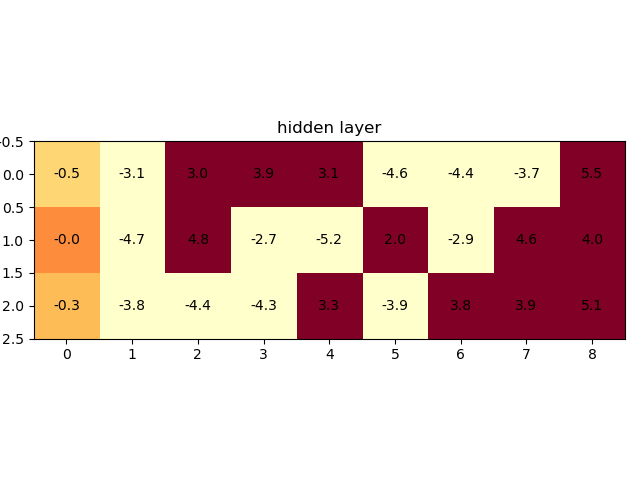
\includegraphics[width=0.5\textwidth]{weights_hidden.png}
    \caption{Weights in hidden layer}
    \label{fig:weights_hidden}
\end{figure}

\begin{figure}
    \centering
    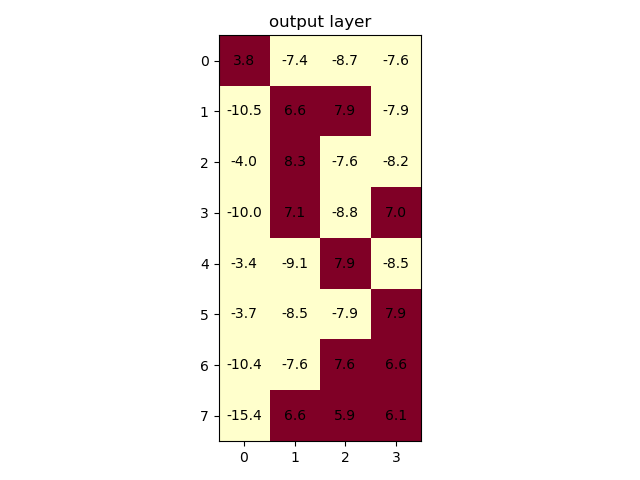
\includegraphics[width=0.6\textwidth]{weights_output.png}
    \caption{Weights in output layer}
    \label{fig:weights_output}
\end{figure}

\begin{figure}
    \centering
    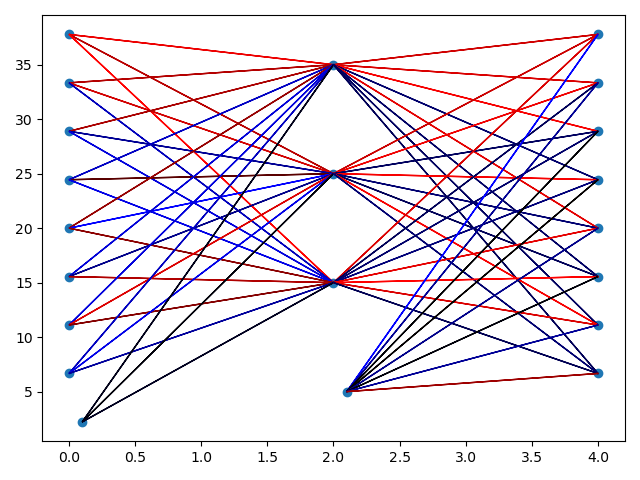
\includegraphics[width=0.6\textwidth]{NN.png}
    \caption{Visualization of the neural network}
    \label{fig:NN_visualized}
\end{figure}




%\section{Summary and Conclusions}
%Add your summary and conclusions here.


\end{document}